% ----------------------------------------------------------
% Fundamentação Teórica
% ----------------------------------------------------------
\chapter{Fundamentação Teórica} \label{cha:fundamentacao}

Neste capítulo serão apresentados os conceitos teóricos utilizados como base para a proposição e desenvolvimento deste trabalho.

\section{Dispositivos móveis e aplicativos híbridos}

Segundo \citeauthor{b2005mobile}, sistemas computacionais móveis são sistemas que podem facilmente ser movidos fisicamente ou cujas capacidades podem ser utilizadas enquanto eles estão sendo movidos. Como estes sistemas preveem tal mobilidade, terminam por oferecer recursos e características que não encontramos em sistemas comuns, como por exemplo: preocupação com nível de energia, armazenamento de dados local/remoto e comunicação com outros sistemas.

Os sistemas computacionais móveis, são desenvolvidos para rodar em celulares, tablets e similares. Para um entendimento mais simples: dispositivo ou sistema móvel deve oferecer a possibilidade de acesso imediato e com o usuário em movimento.

De acordo com um artigo publicado pelo \citeauthor{firstmobile}, a ideia de lançar o primeiro telefone móvel surgiu em 1947 quando um grupo de pesquisadores resolveu melhorar a forma de comunicação a distância. Como naquela época não havia tecnologia suficiente,  essa ideia só saiu do papel em 1973 quando a Motorola, empresa de telecomunicações multinacional americana, apresentou o primeiro aparelho realmente móvel e portátil, DynaTAC 8000X. 

Dos anos 90 para os dias atuais muita coisa mudou numa  velocidade muitíssimo rápida. As tecnologias de transmissão evoluíram e passaram a ser digitais, os equipamentos ficaram menores e muito mais eficientes. Os dispositivos móveis tornaram-se uma ferramenta tão eficiente que deixaram de ser utilizados apenas para ligações e envio de mensagem de texto, se tornando parte integrante da vida moderna em todo o mundo, como pode ser visto na Figura \ref{fig:figura3} 

\begin{figure}[H]
	\caption{\label{fig:figura3}Usuários de dispositivos móveis em todo mundo}
	\centering
	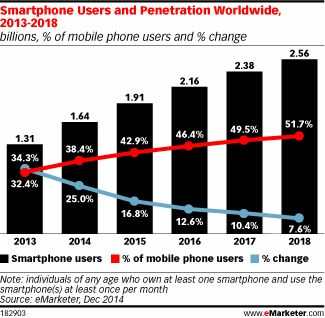
\includegraphics[scale=0.5]{imagens/figura3.jpg}
	\legend{Fonte: \citeauthor{eMarketer}}
\end{figure}

Os dispositivos móveis funcionam juntamente com um sistema operacional. Esse sistema é a plataforma de interação entre o usuário e o dispositivo, onde todos os seus aplicativos serão armazenados e irão funcionar. Hoje, no mercado, há alguns sistemas que se destacam pela qualidade e popularidade, os mais conhecidos são: Android do Google (93,2\% no Brasil e 55,3\% nos Estados Unidos) e IOS da Apple (6,3\% no Brasil e 43,9\% nos Estados Unidos), números baseados numa pesquisa feita pela empresa de analise de dados \citeauthor{kantar}, realizada em 2017. As companhias de tecnologia que desenvolvem os sistemas operacionais disponibilizam Kits de Desenvolvimento de Software (SDK) que permitem aos desenvolvedores criarem e comercializarem milhares de aplicativos com as mais inúmeras funcionalidades em suas lojas virtuais. 

Cada sistema operacional possui a sua própria arquitetura, o que exige o desenvolvimento de aplicações com tecnologias nativas que consigam explorar os seus potenciais específicos. Normalmente, isso implica em linguagens de programação, ferramentas e processos de distribuição específicos (mas não restritos) daquela plataforma. Para um aplicativo nativo do sistema operacional IOS, por exemplo, você precisaria utilizar um Mac, XCode como IDE e desenvolveria em Objetive-C ou Swift.  Por sua vez, um aparelho que tenha como sistema operacional Android poderia ser mais flexível quanto ao computador, mas provavelmente usaria Java como linguagem e o Android Studio como IDE. A Figura \ref{fig:figura4} mostra um pouco essa diferença.

\begin{figure}[H]
	\caption{\label{fig:figura4}Conceito da junção do aplicativo nativo com a aplicação web.}
	\centering
	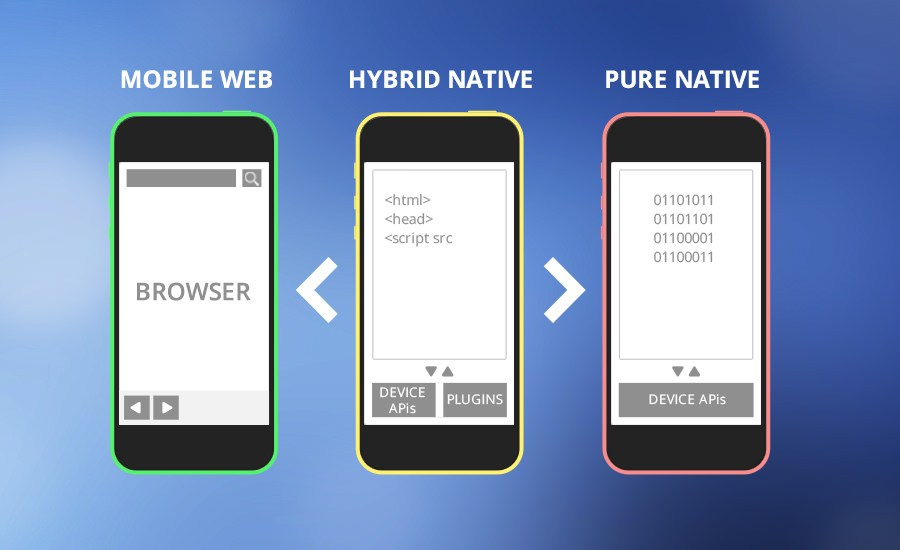
\includegraphics[scale=0.5]{imagens/figura4.jpg}
	\legend{Fonte: Google images}
\end{figure}

Webview é um componente nativo dos sistemas operacionais, que é executado assim que o aplicativo é aberto pelo usuário e contém apenas o necessário para que o aplicativo em HTML5, CSS e JavaScript funcione, se comportando como um motor de renderização do aplicativo, permitindo que tenhamos muito mais recursos do que uma simples página web. 

O desenvolvimento de um aplicativo híbrido acaba sendo mais rápido e também mais barato. A redução de tempo em comparação aos aplicativos nativos se deve à possibilidade de execução do aplicativo híbrido em diferentes plataformas. Devido a essa característica, não há a necessidade de desenvolver o aplicativo várias vezes para se adequar a distintas plataformas, gerando menos impacto sobre o orçamento. Muitas empresas também optam pelo desenvolvimento de aplicativo híbrido em situações que não exigem uma alta performance do aplicativo ou quando o público-alvo é heterogêneo. Nesses casos, uma solução mais genérica para ser usada em plataformas variadas se torna mais vantajosa. A tabela 2 mostra um comparativo entre aplicativos híbridos e nativos.

\begin{table}[H]
	\centering
	\caption{Comparativo entre aplicativos híbridos e nativos.}
	\label{tabela-comparativo-aplicativos-hibridos-nativos}
	\begin{tabular}{|l|c|c|c|}
	\hline
	\textbf{} & \textbf{Híbridos} & \textbf{Nativo (Android / Ios)} & \textbf{Melhor} \\ \hline
	Gráfico & HTML, Canvas, SVG & APIs Nativas & \begin{tabular}[c]{@{}l@{}} Nativo\end{tabular} \\ \hline
	Performance & Lenta & Rápida & \begin{tabular}[c]{@{}l@{}} Nativo\end{tabular} \\ \hline
	Aparência & Emulado & Aparência real & \begin{tabular}[c]{@{}l@{}} Nativo\end{tabular} \\ \hline
	Recursos do equipamento & Muita & Total & \begin{tabular}[c]{@{}l@{}} Nativo\end{tabular} \\ \hline
	Publicação nas lojas & Quase normal & Normal & \begin{tabular}[c]{@{}l@{}} Híbrido\end{tabular} \\ \hline
	Reutilização do código & Total & Nenhuma & \begin{tabular}[c]{@{}l@{}} Híbrido\end{tabular} \\ \hline
	Custo de desenvolvimento & Médio & Alto & \begin{tabular}[c]{@{}l@{}} Híbrido\end{tabular} \\ \hline
	Tempo de desenvolvimento & Baixo & Alto & \begin{tabular}[c]{@{}l@{}} Híbrido\end{tabular} \\ \hline
	Facilidade de atualização & Fácil & Médio & \begin{tabular}[c]{@{}l@{}} Híbrido\end{tabular} \\ \hline
	Conhecimentos requeridos & HTML5, CSS e Javascript & Java, ObjectiveC e Swift & \begin{tabular}[c]{@{}l@{}} Híbrido\end{tabular} \\ \hline
	Curva de aprendizado & Média & Lenta & \begin{tabular}[c]{@{}l@{}} Híbrido\end{tabular} \\ \hline
	
	\end{tabular}
\end{table}


\section{Redes sociais}

Os seres humanos são sociais por natureza, vivem em comunidades, rodeados por outras pessoas. O compartilhamento de informações e interesses entre elas mesmas, são características marcantes da rede social, conhecimentos dos mais diversos tipos, instigam as pessoas a partilhar essas informações e irem a procura de novos conceitos e ideias.

As pessoas estão inseridas em uma sociedade com base nos relacionamentos que desenvolvem durante toda a vida. Estes relacionamentos partilham conhecimento e interesses em comum. As redes sociais são compostas por pessoas (ou organizações) conectadas através destes laços sociais \citeauthor{watts2003}. Com à internet, as redes sociais vêm conquistando cada vez mais adeptos, reunindo pessoas com os mais diversos objetivos e possibilitando a ampliação da sua rede de  relacionamento com pessoas conhecidas ou não, dos mais diversos tipo e lugares, aumentando ainda mais e facilitando a aquisição e compartilhamento de novidades. Como em todo grupo social, existem padrões de comportamento e naturalmente, todas as atitudes consideradas ruins pela comunidade excluem os usuários que o fazem e as atitudes consideradas boas trazem retorno positivo, como uma espécie de recompensa. É importante também que haja um esforço para tentar evitar que usuários e conteúdos falsos sejam criados, para que a credibilidade em geral não seja perdida. Com base nesses conceitos, as redes sociais foram potencializadas através de aplicações web e aplicativos móveis que facilitaram a integração dos seus usuários e estão em crescente uso e expansão, oferecendo diferentes tipos de serviço dependendo das necessidades e preferências dos usuários. Existem redes para fazer negócios, fazer contato com amigos e familiares, conhecer novas pessoas, compartilhar informações. 

Cada uma das redes sociais tem um objetivo, forma e conteúdo diferentes. A sociedade precisa entender e adaptar-se a cada uma delas, buscar ter uma conteúdo que esteja de acordo com a essência de cada uma. Hoje,  as possibilidades são imensas: blogs, locais  de compartilhar musicas, vídeos, de pesquisa, consulta. Na Figura \ref{fig:figura5}, mostramos as principais redes sociais com os seus respectivos números de usuários: 

\begin{figure}[H]
	\caption{\label{fig:figura5}Principais redes sociais com seus respectivos usuários.}
	\centering
	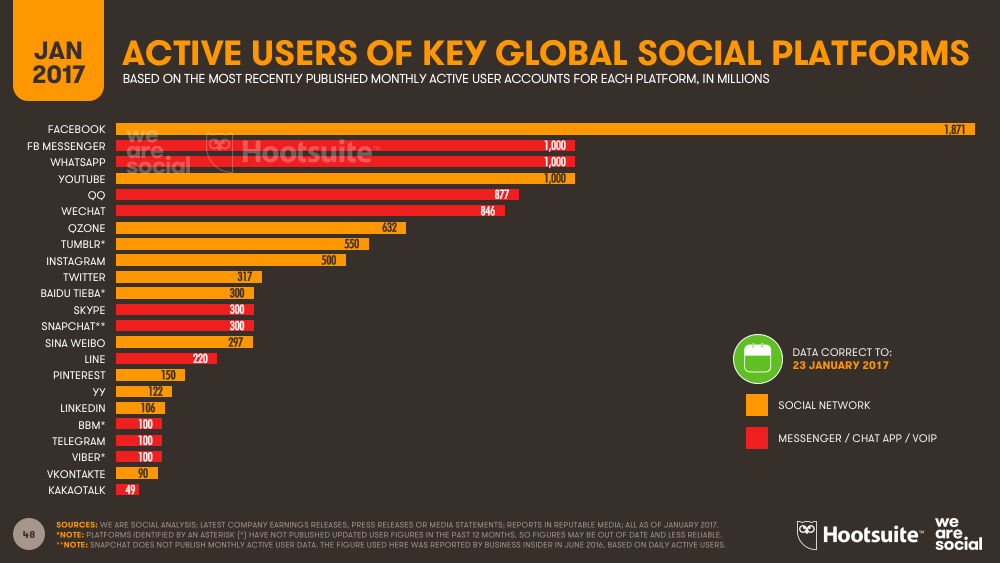
\includegraphics[scale=0.5]{imagens/figura5.png}
	\legend{Fonte: \citeauthor{wearesocial}}
\end{figure}

Baseado na quantidade de usuários utilizando as mais diversas redes sociais, é possível perceber a grande penetração da internet na população mundial e consequentemente podemos observar o grande poder que as redes sociais possuem. Tendo isso em vista, as empresas de diversas áreas acabam investindo cada vez mais nesse mercado que só cresce. Dependendo do público e alcance, investir nas redes sociais acaba sendo uma maneira rápida, fácil e barata de conquistar espaço nesse mercado.

No Brasil, varias empresas estão presentes em pelo menos uma rede social. A presença nas redes sociais acaba sendo um facilitador em entrar em contato com seu publico podendo assim atender as necessidades dos mesmos com uma maior facilidade, aumentando a divulgação dos seus produtos e conquistando novos usuários.

\section{Vegetarianismo}

O vegetarianismo surgiu há cerca de 5 milhões de anos atrás. O
antepassado mais antigo do homem, o Australopithecus Anamensis, alimentava-se
somente de frutas, folhas e sementes, vivendo em perfeita harmonia com os
menores animais, que poderia facilmente apanhar para se alimentar. O domínio do
fogo e o desenvolvimento das armas vêm mudar essa realidade, onde o Homo
Neanderthalensis, caçava, em grupos de 10 a 15, animais de grande porte como os
mamutes e outros de pequeno porte como os veados, dos quais tudo era
meticulosamente aproveitado. Mais tarde, as populações humanas foram criando
culturas de vegetais fixas, que começaram a atrair animais como porcos selvagens,
ovelhas, cães, cabras, aves, ratos e pequenos felinos, que foram sendo
domesticados. Alguns animais começaram a ser mortos para consumo. Foi então
que o homem se tornou sedentário e começou a encarar os animais como alimentos
(\citeauthor{rodrigues2005}, 2005).


Segundo \citeauthor{couceiro2008}(2008, p.365), para que se entenda a origem do vegetarianismo, diz que “o vegetarianismo tem suas origens desde os primórdios da criação do homem e um de seus registros mais amplamente reconhecidos é encontrado no Velho Testamento, na passagem em que Deus diz a Adão e Eva qual deveria ser seu alimento. “

O vegetarianismo tem como premissa a prática de comer alimentos derivados das plantas e não usufruindo de alimentos derivados de origem animal. Com a crescimento do conhecimento e informações sobre os benefícios dos vegetais à saúde, as pessoas passaram a ver a dieta vegetariana como uma melhoria da qualidade de vida. A tabela 3, mostra os países com as maiores taxas de vegetarianismo.


\begin{table}[H]
	\centering
	\caption{Países com as mais altas taxas de vegetarianismo}
	\label{paises-com-as-mais-altas-taxas-de-vegetarianimos}
	\begin{tabular}{|c|c|c|}
	\hline
	\textbf{Classificação} & \textbf{Países com as mais altas taxas de vegetarianismo} & \textbf{Prevalência} \\ \hline
	1  & Índia & 38\% \\ \hline
	2  & Israel & 13\% \\ \hline
	3  & Taiwan & 12\% \\ \hline
	4  & Itália & 10\% \\ \hline
	5  & Áustria & 9\% \\ \hline
	6  & Alemanha & 9\% \\ \hline
	7  & Reino Unido & 9\% \\ \hline
	8  & Brasil & 8\% \\ \hline
	9  & Irlanda & 6\% \\ \hline
	10 & Austrália & 5\% \\ \hline
	\end{tabular}
\end{table}

Segundo \citeauthor{worldatlas2017}, as influências religiosas e culturais contribuem para os altos níveis de vegetarianismo da Índia em relação às normas globais. No caso de Israel, apenas 13\% do seu povo é formado por vegetarianos, influenciados por princípios relacionados com a religião. Os judeus tradicionais obedecem às leis dietéticas kashrut que defendem que um intervalo de seis horas deve ser mantido entre o consumo de leite e carne. Em Taiwan, 12\% da população são vegetarianos, influenciados pela culinárias, religiosidade e fatores governamentais. No caso da Itália tem a maior percentagem de vegetarianos encontrados na União Europeia. A Áustria, Reino Unido e Alemanha contam 9\% de sua população como vegetarianos, ambos com influências sociais e culinárias, apesar de que a Alemanha tem sua reputação como um país amante da carne.  No Brasil, 8\% da população é vegetariana, as influências culinárias e econômicas podem ter sido um fator no vegetarianismo no Brasil. A Irlanda conta com cerca de 6\% de vegetarianos em relação à população total. 5\% dos australianos seguem uma dieta vegetariana.

De uma forma genérica, o vegetarianismo é um regime alimentar que exclui da dieta todos os tipos de carne, bem como todos alimentos derivados. É baseado fundamentalmente no consumo de alimento de origem vegetal, com ou sem o consumo de laticínios e/ou ovos. Ovos e laticínios, embora sejam de origem animal, estão incluídos na dieta de alguns vegetarianos. Por essa e outras diferenças, que os vegetarianos são sendo categorizados em 4 grupos principais citados na Figura \ref{fig:figura6}.

\begin{figure}[H]
	\caption{\label{fig:figura6}Tipos de vegetarianos.}
	\centering
	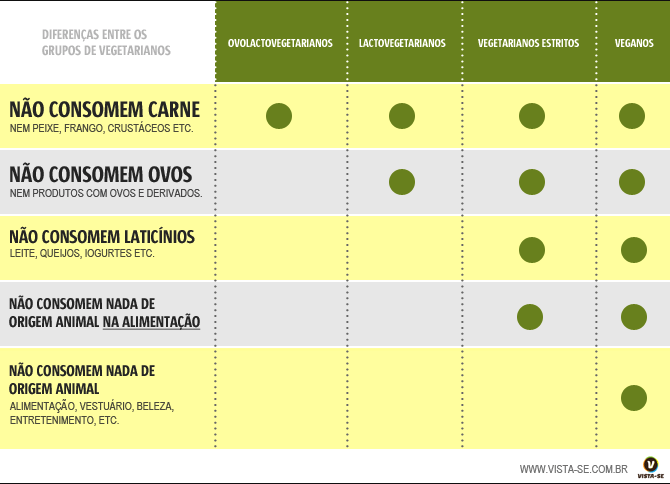
\includegraphics[scale=0.5]{imagens/figura6.png}
	\legend{Fonte: \citeauthor{tiposveggies}}
\end{figure}

Nas redes sociais, o vegetarianismo e veganismo tem ganho cada vez mais popularidade. Apesar de terem muitas semelhanças, ambos tem algumas diferenças, criando uma identidade completamente diferentes para os indivíduos que fazem parte destes grupos. Enquanto o vegetarianismo tem por sua base a alimentação, em não consumir nada de origem animal e derivados, o veganismo tem uma premissa mais ética, a luta pela libertação e não exploração animal, além da alimentação, os veganos não usufruem de nada de origem animal, incluindo roupas, cosméticos e remédios. Por isso os veganos estão sempre atentos sobre as empresas que fazem produtos e/ou testes em animais, buscando outras alternativas 

De acordo com aqueles que adotam a postura vegana, os animais não devem ser mortos e nem explorados para atender às nossas necessidades. A prática do veganismo vem carregada de sacrifícios e vontades negadas. 